\section{Gibbs and the Reification of Vectors: From Geometry Back to Calculation}


\subsection{The Leap from Riemann to Gibbs}

If Riemann revealed that space itself could curve,  
and Cayley abstracted geometry into algebra,  
and Fourier decomposed phenomena into modes,  
then Josiah Willard Gibbs gave scientists a way to calculate with these abstractions in their hands.

Where Riemann turned geometry into a field of tensors and manifolds,  
Gibbs brought geometry back to the working desk of the physicist—  
transforming mathematical abstraction into a usable calculus for fields, forces, and flows.

Riemann had given us a vision: space as a manifold, geometry as curvature, distances defined intrinsically by a metric.

But in the 19th century, physics still operated largely in the Euclidean world of three-dimensional space.

Physicists needed tools to work with fields, forces, and rotations—  
to describe electromagnetism, fluid dynamics, and mechanics without drowning in the expanding 
notational machinery of quaternions or matrix algebras.

It was here that Gibbs intervened by introducing \textbf{vector analysis}: a system where vectors could be manipulated by clear operations tied 
directly to physical meaning:

He recognized physicists mostly needed operations in three dimension
\begin{itemize}
    \item dot products: $\vec{A} \cdot \vec{B}$, 
    \item cross products: $\vec{A} \times \vec{B}$, 
    \item gradients: $\nabla$, 
    \item divergences $\nabla \cdot \vec{F}$, and
    \item curls: $\nabla \times \vec{F}$.
\end{itemize}

Gibbs stripped the machinery down to what was essential.  His goal was to give physicists “tools for calculation” 
so they could focus on physical insight rather than wrestle with more cumbersome algebraic frameworks.

\medskip

\begin{HistoricalSidebar}{Reification in Gibbs’s Vector Analysis}

    In philosophy and mathematics, \emph{reification} is the process of turning an abstract concept into a concrete object—“thingifying” ideas so they can be manipulated directly.  From Plato’s Forms to modern abstract algebra, thinkers have sought ways to handle abstractions as tangible entities.

    \medskip
    
    Gibbs’s great insight was to \textbf{reify} the intricate tensorial and analytical machinery of Riemannian geometry and Hamilton’s quaternions into the familiar objects of three-dimensional vector space:

    \medskip
    
    \begin{itemize}
      \item \textbf{Abstract curvature and tensor fields} became the \emph{vector field} \(\vec F(x,y,z)\), a concrete list of components.
      \item \textbf{Coordinate‐free differential operators} were reified as the gradient \(\nabla\), divergence \(\nabla\!\cdot\), and curl \(\nabla\times\)—literal formulas that physicists could write and compute.
      \item \textbf{Complex quaternionic rotations} were distilled into the cross product \(\vec A\times\vec B\), a simple determinant.
    \end{itemize}

    \medskip
    
    By reification, Gibbs provided a \emph{calculus of things} --- vectors and operations on them --- so that what once lived in abstract algebraic structures could be handled by straightforward symbol manipulation.  His vector analysis became the lingua franca of physics, demonstrating that the power of deep abstraction is unlocked only when it is given a concrete form fit for computation.

\end{HistoricalSidebar}


\subsection{From Metric Tensors to Concrete Components: A Point‐by‐Point Comparison}

\subsubsection{Dot Product}
In an indexed formulation, the inner product of two vectors \(A\) and \(B\) in arbitrary coordinates is written
\[
g_{ij}\,A^i\,B^j,
\]
where \(g_{ij}\) represents how lengths and angles are measured in those coordinates.  Gibbs observed that in flat, Cartesian space the metric is simply the identity, so the same calculation reduces to
\[
\vec A\cdot\vec B
= A_x\,B_x + A_y\,B_y + A_z\,B_z.
\]
Physicists no longer needed to carry around a table of metric components—just three multiplications and two additions.


\begin{figure}[H]
    \centering
    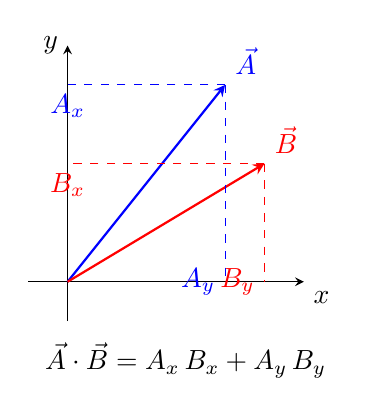
\begin{tikzpicture}[>=stealth, scale=1]
      % Origin
      \coordinate (O) at (0,0);
      % Vectors
      \coordinate (A) at (2,2.5);
      \coordinate (B) at (2.5,1.5);
    
      % Axes
      \draw[->] (-0.5,0) -- (3,0) node[below right] {$x$};
      \draw[->] (0,-0.5) -- (0,3) node[left] {$y$};
    
      % Vectors A and B
      \draw[->, thick, blue] (O) -- (A) node[above right] {$\vec A$};
      \draw[->, thick, red]  (O) -- (B) node[above right] {$\vec B$};
    
      % Projections of A
      \draw[dashed, blue] (A) -- (A -| O) node[below] {$A_x$};
      \draw[dashed, blue] (A) -- (A |- O) node[left]  {$A_y$};
    
      % Projections of B
      \draw[dashed, red]  (B) -- (B -| O) node[below] {$B_x$};
      \draw[dashed, red]  (B) -- (B |- O) node[left]  {$B_y$};
    
      % Dot‐product formula
      \node at (1.5,-1) {\(\displaystyle \vec A\cdot\vec B = A_x\,B_x + A_y\,B_y\)};
    \end{tikzpicture}
    \caption{Component‐wise interpretation of the dot product in Cartesian coordinates.}
\end{figure}





\subsubsection{Cross Product}
Before Gibbs, rotations and oriented areas were often handled by quaternions or by antisymmetric two–index objects.  Gibbs distilled the idea into the familiar determinant
\[
\vec A\times\vec B
=\begin{vmatrix}
\hat i & \hat j & \hat k\\
A_x    & A_y    & A_z\\
B_x    & B_y    & B_z
\end{vmatrix},
\]
so that torques and magnetic forces could be computed by memorizing one \(3\times3\) rule instead of wrestling with more abstract algebraic systems.


\begin{figure}[H]
    \centering
    \begin{tikzpicture}[scale=1.2]
      % Coordinates
      \coordinate (O) at (0,0);
      \coordinate (A) at (2,1);
      \coordinate (B) at (1,2);
      \coordinate (C) at ($(A)+(B)$);
    
      % Axes
      \draw[->] (-0.5,0) -- (3,0) node[below] {$x$};
      \draw[->] (0,-0.5) -- (0,3) node[left] {$y$};
    
      % Vectors A and B
      \draw[->, thick, blue]  (O) -- (A) node[above right] {$\vec A$};
      \draw[->, thick, red]   (O) -- (B) node[above left]  {$\vec B$};
    
      % Parallelogram spanned by A and B
      \fill[blue!20] (O) -- (A) -- (C) -- (B) -- cycle;
      \draw[dashed] (A) -- (C) -- (B);
    
      % Cross product arrow (out of page)
      \draw[->, very thick, purple] ($(O)!0.5!(C)$) -- ++(0,0.8) node[right] {$\vec A\times\vec B$};
      \node at ($(O)!0.5!(C)+(0,0.8)$) {\Large\(\odot\)};
      \node at ($(O)!0.5!(C)+(0,0.6)$) {\small (out of page)};
    
    \end{tikzpicture}
    \caption{The cross product \(\vec A\times\vec B\) is perpendicular to the parallelogram spanned by \(\vec A\) and \(\vec B\).}
\end{figure}






\subsubsection{Gradient}
In component notation on any coordinate grid, one writes
\[
(\nabla f)_i = \frac{\partial f}{\partial x^i},
\]
leaving open how those components relate to physical lengths.  Gibbs fixed the grid to Cartesian axes and simply set
\[
\nabla f
= \Bigl(\tfrac{\partial f}{\partial x},\,\tfrac{\partial f}{\partial y},\,\tfrac{\partial f}{\partial z}\Bigr),
\]
freeing practitioners from transformations between coordinate bases.


\begin{figure}[H]
    \centering
    \begin{tikzpicture}[scale=1.2,>=stealth]
      % Axes
      \draw[->] (-0.5,0) -- (2.5,0) node[below right] {$x$};
      \draw[->] (0,-0.5) -- (0,2.5) node[left] {$y$};
    
      % Level curves (contours) of a sample function f(x,y)
      \draw[dashed] (0,0) circle (1);
      \draw[dashed] (0,0) circle (1.5);
      \draw[dashed] (0,0) circle (2);
    
      % Point where gradient is evaluated
      \coordinate (P) at (1,1);
      \fill (P) circle (1.5pt) node[above left] {$(x_0,y_0)$};
    
      % Gradient vector at P
      \coordinate (G) at ($(P)+(0.6,0.4)$);
      \draw[->, thick, red] (P) -- (G) node[above right] {$\nabla f$};
    
      % Projections of gradient onto axes
      \coordinate (Hx) at (1.6,1);
      \coordinate (Vy) at (1,1.4);
      \draw[dashed] (G) -- (Hx);
      \draw[dashed] (G) -- (Vy);
    
      % Partial derivative components
      \draw[->, blue] (P) -- (Hx) node[midway, below] {$\displaystyle \frac{\partial f}{\partial x}$};
      \draw[->, blue] (P) -- (Vy) node[midway, left]  {$\displaystyle \frac{\partial f}{\partial y}$};
    
    \end{tikzpicture}
    \caption{Visualization of the gradient \(\nabla f = \bigl(\partial_x f,\partial_y f\bigr)\) at a point \((x_0,y_0)\).}
\end{figure}







\subsubsection{Divergence}
Abstractly, divergence is the contraction of a derivative with a vector,
\[
\nabla_i F^i = \frac{\partial F^i}{\partial x^i},
\]
with the understanding that one must track how volume elements change under coordinate transformations.  In Cartesian form, Gibbs collapsed this to
\[
\nabla\!\cdot\vec F
= \tfrac{\partial F_x}{\partial x}
+ \tfrac{\partial F_y}{\partial y}
+ \tfrac{\partial F_z}{\partial z},
\]
a single, coordinate‐fixed sum of partial derivatives measuring net outflow per unit volume.

\begin{figure}[H]
    \centering
    \begin{tikzpicture}[>=stealth, scale=1]
      % Small box representing a volume element
      \draw (0,0) rectangle (2,2);
    
      % Arrows on right and left faces (F_x)
      \draw[->, thick] (2,0.5) -- ++(0.6,0) node[right] {$F_x(x+\Delta x)$};
      \draw[->, thick] (0,1.5) -- ++(-0.3,0) node[left] {$F_x(x)$};
    
      % Arrows on top and bottom faces (F_y)
      \draw[->, thick] (0.5,2) -- ++(0,0.6) node[above] {$F_y(y+\Delta y)$};
      \draw[->, thick] (1.5,0) -- ++(0,-0.3) node[below] {$F_y(y)$};
    
      % Label for the box
      \node at (1,1) [font=\small] {$\Delta V$};
    \end{tikzpicture}
    \caption{Net outflow across a small square: the divergence 
    \(\nabla\!\cdot\vec F\approx\frac{F_x(x+\Delta x)-F_x(x)}{\Delta x}+\frac{F_y(y+\Delta y)-F_y(y)}{\Delta y}\)
    measures how much more fluid leaves than enters per unit volume.}
\end{figure}







\subsubsection{Curl}
The curl in index form is often written by antisymmetrizing partial derivatives,
\[
(\nabla\times F)^i = \frac{\partial F^i}{\partial x^j} - \frac{\partial F^j}{\partial x^i},
\quad\text{for }(i,j)\in\{(1,2),(2,3),(3,1)\}.
\]
Gibbs gave the compact determinant mnemonic
\[
\nabla\times\vec F
=\begin{vmatrix}
\hat i & \hat j & \hat k\\
\partial_x & \partial_y & \partial_z\\
F_x        & F_y        & F_z
\end{vmatrix},
\]
so that circulation and vorticity could be computed in one elegant stroke rather than expanded index by index.

In each case, Gibbs replaced coordinate‐agnostic but index‐heavy formulas with direct component expressions tied to the familiar \(x,y,z\) axes.  The result was a practical calculus of vectors—straightforward to teach, compute, and apply.  


\begin{figure}[H]
    \centering
    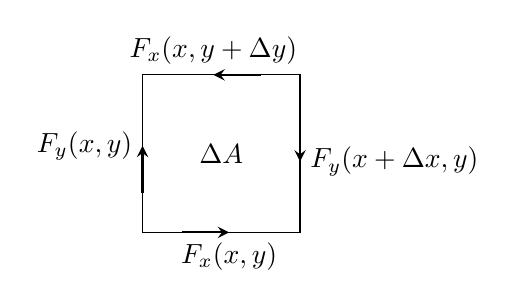
\begin{tikzpicture}[>=stealth, scale=1]
      % Small square representing an area element
      \draw (0,0) rectangle (2,2);
    
      % Arrows on left and right edges (vertical component F_y)
      \draw[->, thick] (0,0.5) -- ++(0,0.6) node[left]  {$F_y(x,y)$};
      \draw[->, thick] (2,1.5) -- ++(0,-0.6) node[right] {$F_y(x+\Delta x,y)$};
    
      % Arrows on bottom and top edges (horizontal component F_x)
      \draw[->, thick] (0.5,0) -- ++(0.6,0) node[below] {$F_x(x,y)$};
      \draw[->, thick] (1.5,2) -- ++(-0.6,0) node[above] {$F_x(x,y+\Delta y)$};
    
      % Label for the square
      \node at (1,1) {$\Delta A$};
    \end{tikzpicture}
    \caption{Circulation around a small square: the net “spin” per unit area 
    \(\displaystyle \frac{F_y(x+\Delta x,y)-F_y(x,y)}{\Delta x}
    - \frac{F_x(x,y+\Delta y)-F_x(x,y)}{\Delta y}
    \approx (\nabla\times \vec F)_z\).}
\end{figure}











\subsection{From Curvature to Calculation}

Where Riemann envisioned spaces bending under curvature,  
Gibbs gave a language to describe the flow of water through a pipe,  
the rotation of a magnetic field,  
the divergence of an electric field from a point charge.

In Gibbs’s vector analysis, physicists could manipulate fields algebraically without invoking coordinates explicitly.  
They could calculate work, circulation, flux, and potential with a symbolic toolkit directly mirroring physical intuition.

In a sense, Gibbs’s leap was a move from **geometry back to calculation**—  
from the grand structures of curved manifolds to the **pragmatic structures of fields living inside \( \mathbb{R}^3 \).**




\medskip

\begin{HistoricalSidebar}{From Quaternions to Vector Calculus}

    Hamilton’s first great algebraic insight came in 1843 with the invention of quaternions, an ambitious extension of complex numbers that bundled a real scalar \(s\) together with a three‐component “vector” \((x,y,z)\) into a single entity
    
    \[
    q = s \;+\; x\,\mathbf i \;+\; y\,\mathbf j \;+\; z\,\mathbf k.
    \]
    
    Quaternion multiplication weaves together both scalar and vector parts, so that in one algebraic stroke you recover:

    \medskip
    
    \begin{itemize}
      \item The \emph{dot product} from the resulting scalar component, and  
      \item The \emph{cross product} from the vector component.  
    \end{itemize}

    \medskip
    
    This unified framework beautifully encodes rotations in three‐dimensional space and foreshadows modern ideas of spin and orientation.  Yet in practice, physicists found the four‐dimensional notation bulky:

    \medskip
    
    \begin{itemize}
      \item One always carried an extra “scalar head” \(s\) even when only vector operations were needed.
      \item The non‐commutative rules (e.g.\ \(\mathbf i\,\mathbf j = \mathbf k\), but \(\mathbf j\,\mathbf i = -\mathbf k\)) were conceptually elegant but cumbersome for everyday calculations.
      \item Writing out quaternion products often obscured the physical meaning behind simple projections and curls.  
    \end{itemize}

    \medskip
    
    In the late 19th century, both Josiah Gibbs and Oliver Heaviside independently recognized that most applications in mechanics, electromagnetism, and fluid dynamics only required the three‐vector machinery.  They:

    \medskip
    
    \begin{itemize}
      \item \emph{Extracted} the vector part of Hamilton’s algebra—abandoning the scalar component when it wasn’t needed.
      \item \emph{Formalized} the dot “\(\cdot\)” and cross “\(\times\)” as primitive operations.
      \item \emph{Introduced} the del operator “\(\nabla\)” to unify gradient, divergence, and curl in one compact symbol.
      \item \emph{Streamlined} notation so that physicists could write \(\vec A \cdot \vec B\) instead of juggling quaternionic products like \(\mathbf A\,\mathbf B + \mathbf B\,\mathbf A\).
    \end{itemize}

    \medskip
    
    The result was a lean, intuitive \emph{vector calculus} tailored to the needs of practitioners: every arrow \(\vec v\) became a concrete 3‐tuple, every operator a direct combination of partial derivatives, and the heavy quaternionic scaffolding was left behind.  In so doing, Gibbs and Heaviside reified Hamilton’s abstract vision into the everyday toolkit of modern physics.
    
\end{HistoricalSidebar}
    


\medskip




\bigskip

\subsection*{A Bridge Between Abstract and Applied}

Gibbs didn’t negate Riemann’s geometry; he gave physicists a working interface with it,  
before tensor calculus became widespread.

His vector analysis acted as a bridge between the geometric abstraction of curvature  
and the hands-on algebra needed for Maxwell’s equations, thermodynamics, and mechanics.

Where Fourier decomposed functions, Gibbs decomposed physical phenomena into components aligned with human measurement—along, across, rotating around.

And where Cayley encoded transformations algebraically, Gibbs encoded physical operations algebraically.

\bigskip

\begin{quote}
In Euler, we computed forces.  
In Lagrange, we minimized action.  
In Hamilton, we traced flows.  
In Jacobi, we found surfaces.  
In Cayley, we abstracted transformations.  
In Fourier, we decomposed vibrations.  
In Riemann, we curved the space.  
In Gibbs, we brought geometry back into the laboratory.
\end{quote}

\subsection*{Setting the Stage for Tensors and Fields}

Gibbs’s system made the manipulation of vectors intuitive,  
but the world would soon require more:  
tools capable of describing fields not just in \( \mathbb{R}^3 \), but in curved spacetime itself.

The simplicity of Gibbs’s dot and cross products would generalize into the tensor calculus of Ricci and Levi-Civita,  
where operations had to work across coordinates that bent and twisted under curvature.

But before tensors were universal, Gibbs gave physicists the algebra they needed to tame vectors.

And in doing so, he laid a practical foundation that would echo even in the curved geometries of Einstein’s universe.


\subsection*{Reinterpreting Kepler’s Second Law Through Gibbs’s Vector Analysis}

Gibbs brought physics back to the chalkboard — and with it, a notation that made celestial mechanics calculable in three dimensions.

Kepler’s Second Law — that a planet sweeps out equal areas in equal times — can now be understood not just as a geometric principle or a curvature-induced symmetry,  
but as a direct consequence of a conserved quantity in vector form.

\bigskip

\begin{tcolorbox}[colback=blue!5!white, colframe=blue!70!black, title=\textbf{Gibbs’s View: Kepler as a Vector Conservation Law}]
In Gibbs’s language, Kepler’s Law is the constancy of the areal velocity vector:
\[
\vec{L} = \vec{r} \times \vec{v}
\quad \text{with} \quad
\frac{d\vec{L}}{dt} = 0
\]
\end{tcolorbox}

\bigskip

\paragraph{From Area Sweep to Angular Momentum.}

The areal velocity swept out by the planet is given by:
\[
\frac{dA}{dt} = \frac{1}{2} \left\| \vec{r} \times \vec{v} \right\|
\]

This is precisely half the magnitude of the angular momentum per unit mass:
\[
\vec{L} = \vec{r} \times m\vec{v}
\]

In Gibbs’s formalism, this isn’t just a geometric fact — it’s an algebraic identity.  
The cross product encodes both the direction of orbital motion and the plane in which the motion is confined.

\bigskip

\paragraph{Why the Cross Product Matters.}

Thanks to Gibbs, we now treat the cross product as a fundamental tool in physics.  
And Kepler’s Law becomes a perfect example of its meaning:

\begin{itemize}
    \item The direction of \( \vec{r} \times \vec{v} \) is perpendicular to the orbital plane,
    \item The magnitude measures twice the areal velocity,
    \item Its conservation implies that no torque acts perpendicular to the plane.
\end{itemize}

In short, the vector remains constant — and that constancy is the Second Law, expressed with precision and power.

\bigskip

\paragraph{From Geometry to Calculation.}

What had once required diagrams and proportional reasoning,  
Gibbs now lets us express in a single algebraic condition:

\[
\vec{r} \times \vec{v} = \text{constant}
\]

This equation is compact, visualizable, and computationally tractable — a gift to physicists navigating real-world orbits.

\bigskip

\begin{quote}
Kepler drew ellipses.  
Newton explained forces.  
Gibbs wrote: \quad \( \vec{r} \times \vec{v} = \text{const} \)  
And every physicist since has smiled.
\end{quote}

\begin{figure}[H]
    \centering
    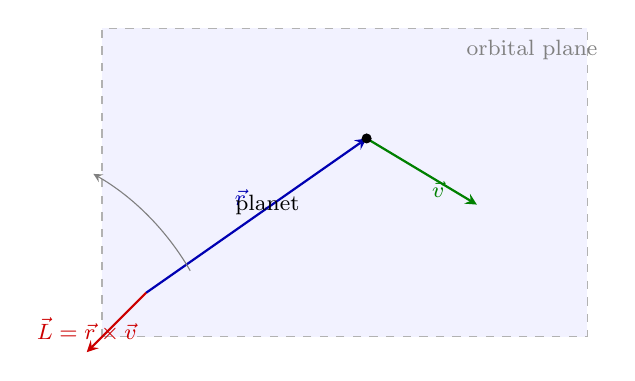
\begin{tikzpicture}[scale=2.8, >=stealth]
    
      % Origin and axes
      \coordinate (O) at (0,0);
      \coordinate (R) at (1,0.7);  % r vector
      \coordinate (V) at (1.2,0.2); % v vector
      \coordinate (L) at (0,0,1); % angular momentum vector (out of plane)
    
      % Draw orbital plane
      \fill[blue!5] (-0.2,-0.2) rectangle (2,1.2);
      \draw[black!30, dashed] (-0.2,-0.2) rectangle (2,1.2);
      \node[black!50] at (1.75,1.1) {\footnotesize orbital plane};
    
      % Vectors
      \draw[->, thick, blue!70!black] (O) -- (R) node[midway, above left] {\footnotesize $\vec{r}$};
      \draw[->, thick, green!50!black] (R) -- ++(0.5,-0.3) node[midway, below right] {\footnotesize $\vec{v}$};
      \draw[->, thick, red!80!black] (O) -- (0,0,0.7) node[above] {\footnotesize $\vec{L} = \vec{r} \times \vec{v}$};
    
      % Add circular arc to show motion
      \draw[black!50, ->] (0.2,0.1) arc[start angle=30, end angle=60, radius=1.2];
    
      % Labels
      \node at (0.55,0.4) {\footnotesize planet};
      \filldraw[black] (R) circle (0.02);
    
    \end{tikzpicture}
    \caption{Visualization of Kepler’s Second Law using Gibbs’s vector notation. The cross product $\vec{r} \times \vec{v}$ yields a constant angular momentum vector perpendicular to the orbital plane.}
    \end{figure}
    